\section{Background}\label{sec:background}

This section introduces the technologies the project builds on. Readers who already know Kubernetes can skip Section~\ref{sec:k8s}.

\subsection{Containers and Kubernetes in five minutes}\label{sec:k8s}

A \textbf{container} is a packaged program together with everything it needs to run (libraries, runtime, configuration). The package is called an \textbf{image}; running an image produces a container. Containers start in seconds and are isolated from each other, which makes them the standard unit of deployment for backend services.

Running one container on one machine is easy (\code{docker run}). Running hundreds of containers on dozens of machines, restarting the ones that crash and spreading load evenly, is not. \textbf{Kubernetes} is the system that does this. The key idea is that you do not tell Kubernetes \emph{what to do}; you tell it \emph{what you want}, in a YAML file, and it keeps the cluster in that state (Figure~\ref{fig:k8s}).

\begin{figure}[H]
  \centering
  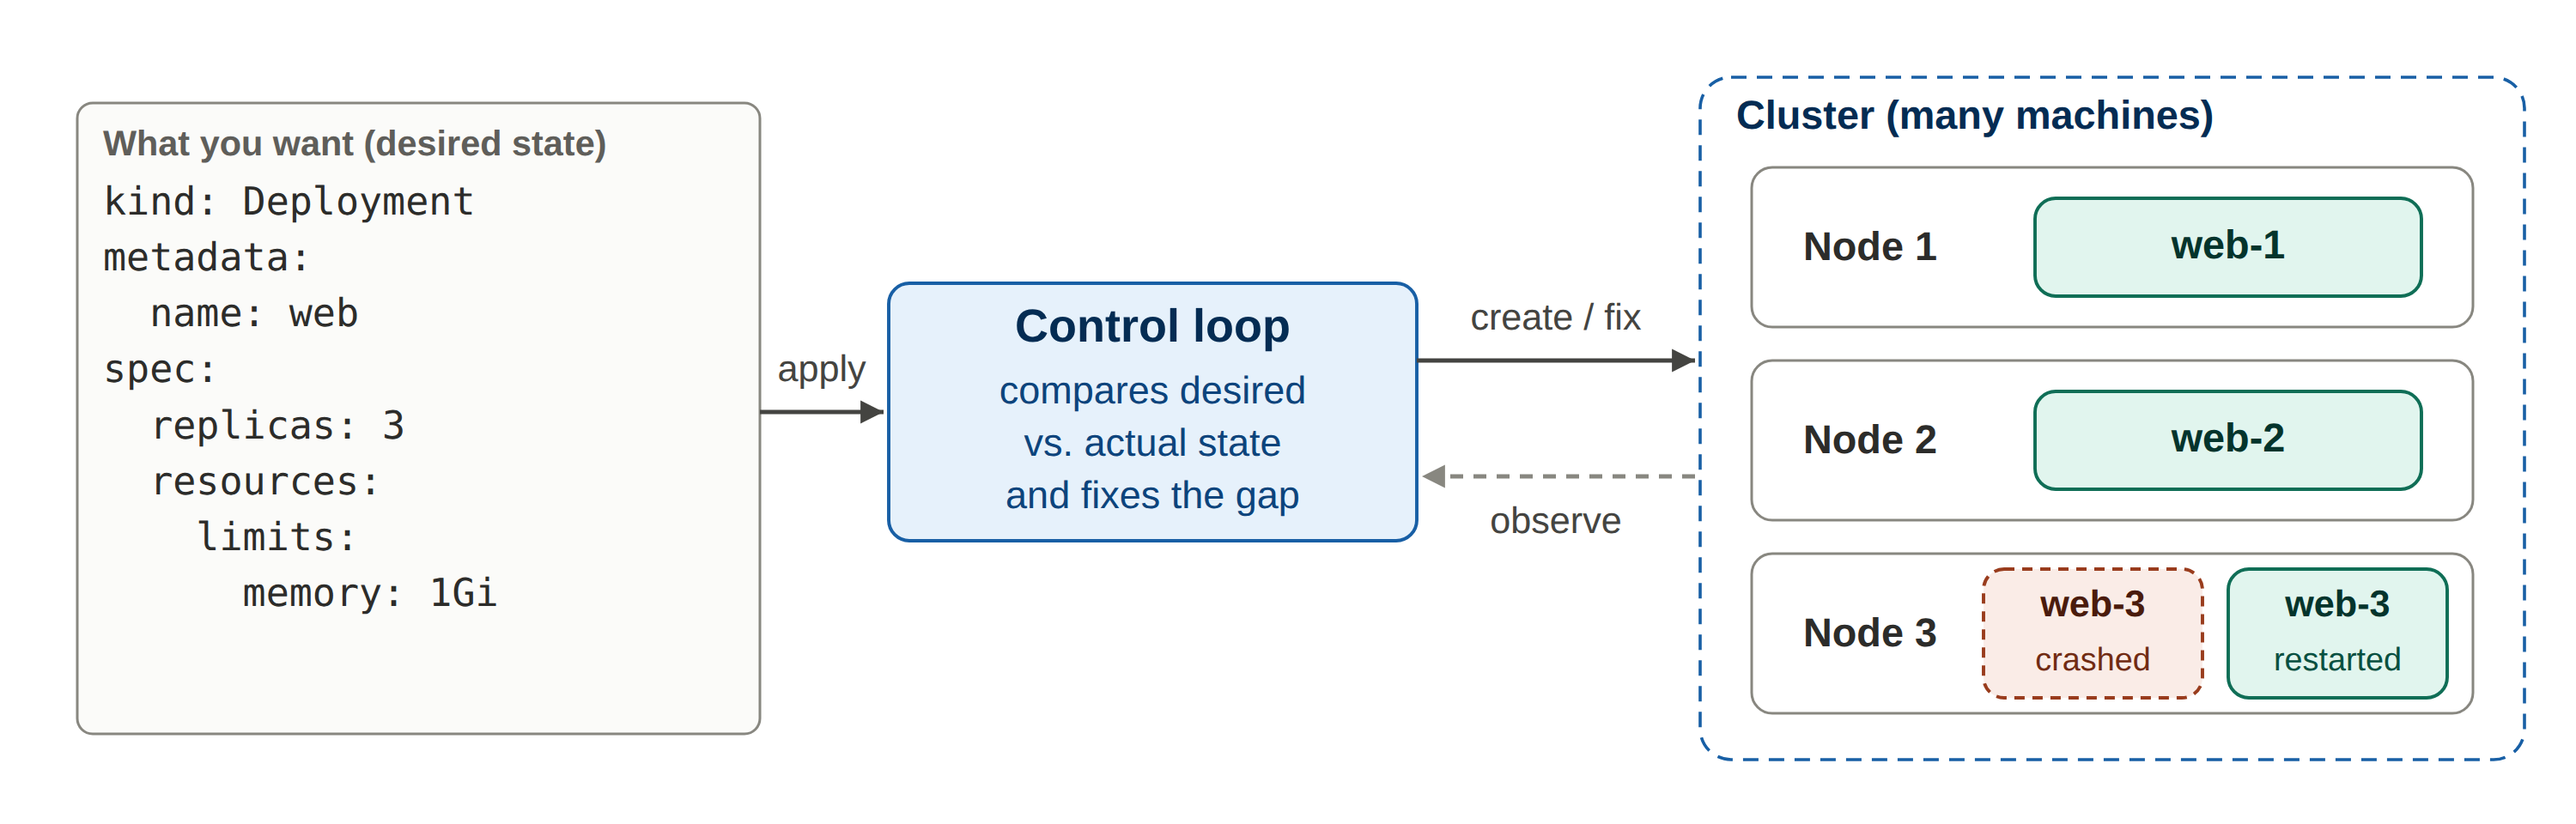
\includegraphics[width=\linewidth]{k8s_declarative.png}
  \caption{Declarative control in Kubernetes. You describe the desired state (here: three copies of a web server with 1~GiB of memory each). A control loop continuously compares it with the actual state and fixes differences, for example by restarting a crashed copy on node~3.}
  \label{fig:k8s}
\end{figure}

A handful of terms is enough to follow the rest of this document:

\begin{center}
\small
\begin{tabularx}{\linewidth}{@{}L{3.1cm}Y@{}}
\toprule
\textbf{Term} & \textbf{Meaning}\\
\midrule
Node & One machine (physical or virtual) in the cluster.\\
Pod & The smallest thing Kubernetes runs: one or more containers scheduled together on a node.\\
Namespace & A named partition of the cluster, used to group and isolate resources.\\
Manifest & A YAML document describing a desired resource (\code{kind}, \code{metadata}, \code{spec}).\\
Controller & A program running a control loop that makes reality match the manifests.\\
Secret & A resource that stores sensitive values (API keys, passwords) and injects them into containers.\\
NetworkPolicy & A rule restricting which pods may talk to which destinations.\\
\code{kubectl} & The command-line client: \code{kubectl apply -f file.yaml}, \code{kubectl get pods}, \ldots\\
\bottomrule
\end{tabularx}
\end{center}

For this project Kubernetes is the ground floor: AX and Agent Substrate are installed on it, and our own components are ordinary Kubernetes services running next to them. We will not need to write Kubernetes controllers ourselves.

\subsection{From a local coding assistant to agents at scale}

Figure~\ref{fig:analogy} compares two ways of running agents. On the left is a familiar setting: a coding assistant on a laptop that delegates work to a few sub-agents. The human is the safety mechanism: the agents act with the human's permissions, and the human watches. On the right is a cluster running agents as \emph{workloads}. There are far more of them, they run unattended, and the safety mechanism has to be built into the platform.

\begin{figure}[H]
  \centering
  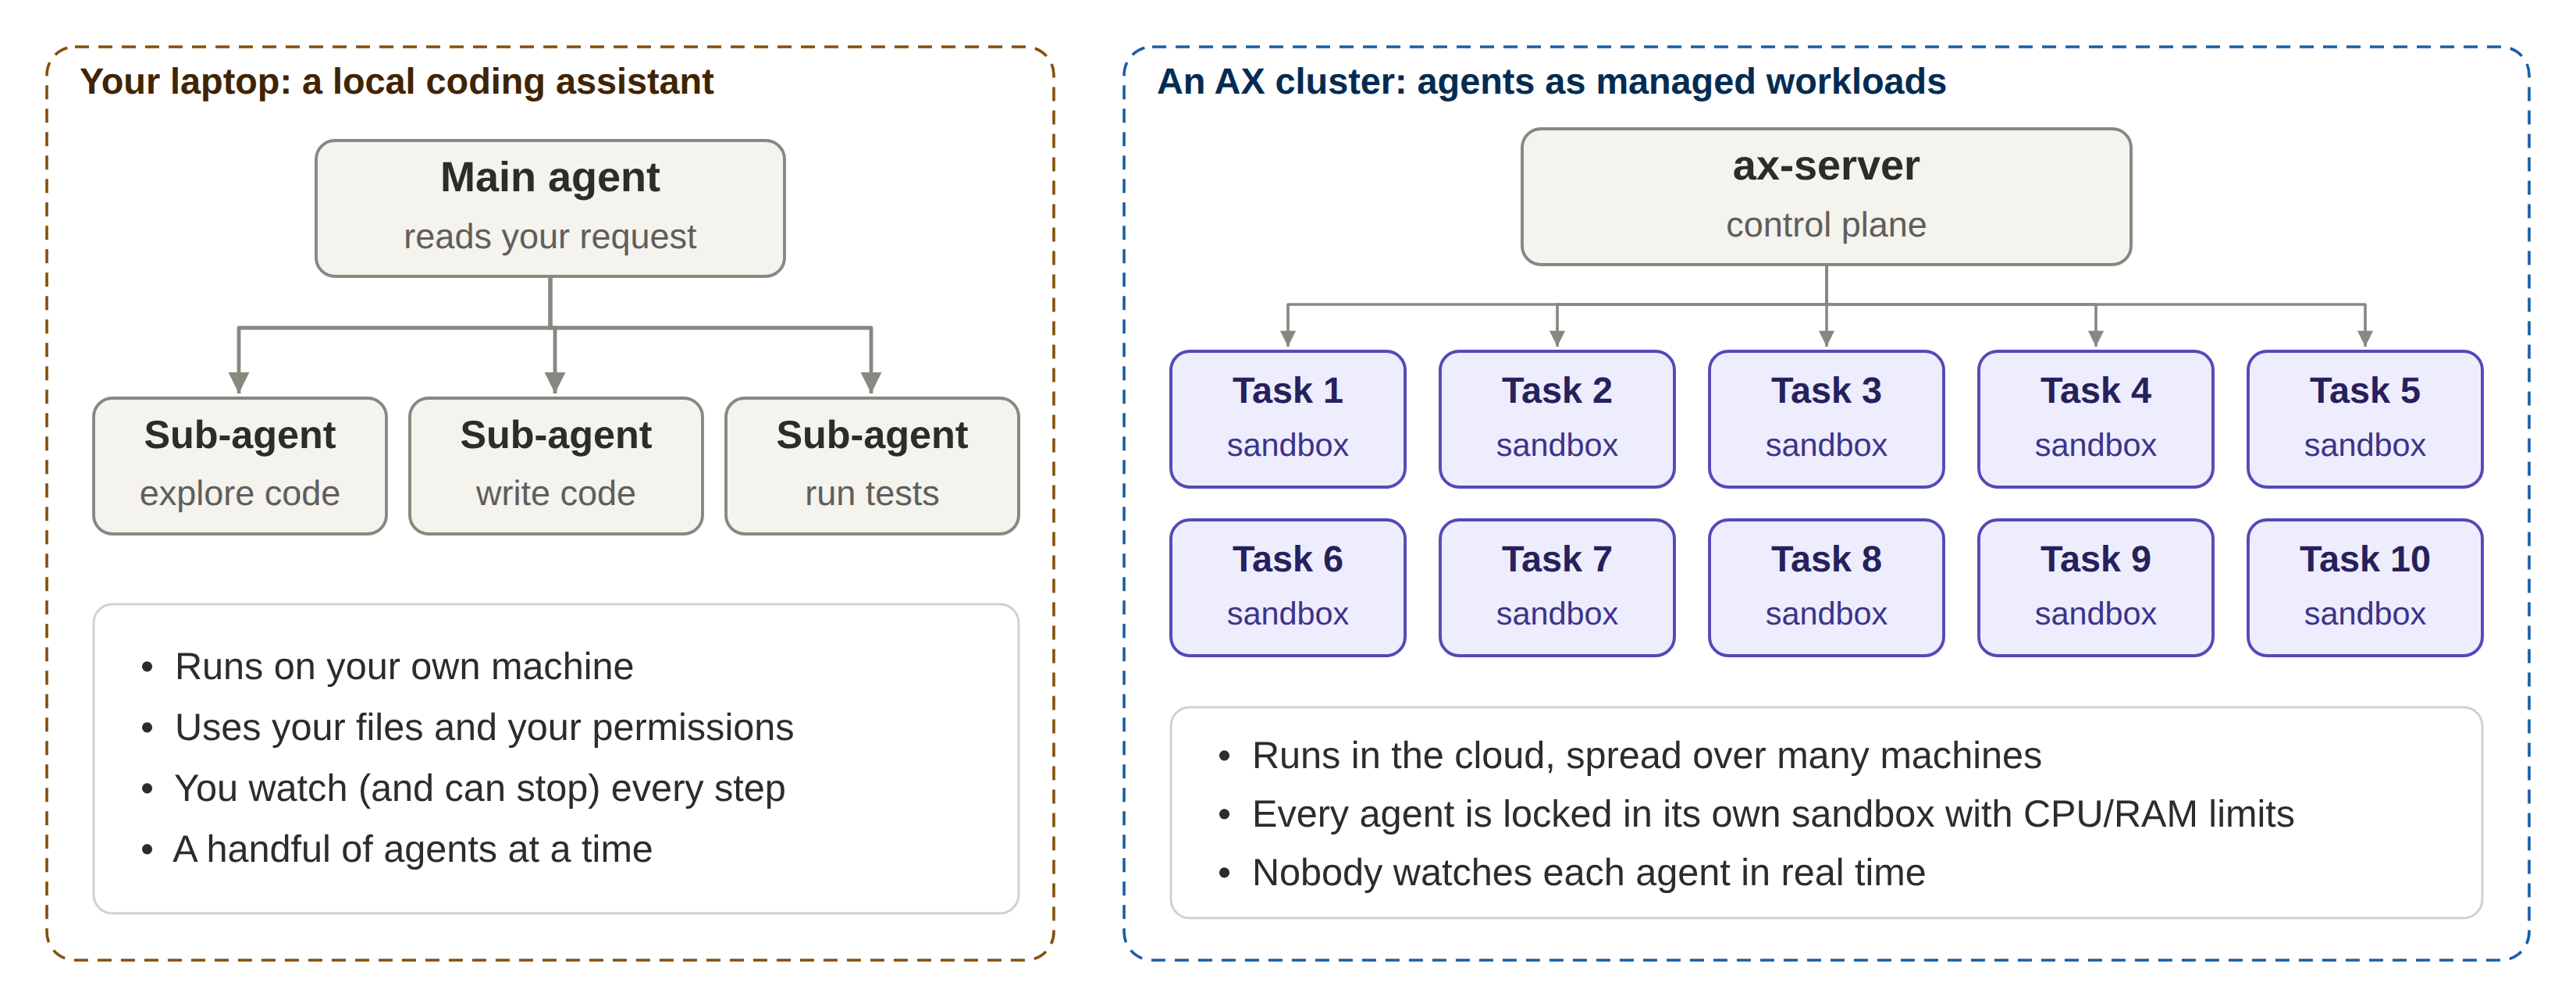
\includegraphics[width=\linewidth]{analogy.png}
  \caption{Local sub-agents versus agents as managed cluster workloads. When nobody is watching each agent, isolation, limits and accountability must come from the platform.}
  \label{fig:analogy}
\end{figure}

Agents are an unusual kind of workload. The AX documentation puts it this way: they ``are neither stateless microservices nor run-to-completion batch jobs. They accumulate state, need strict isolation, call out to model APIs and tool servers, and can burn money in a loop if nobody is watching''~\cite{ax}. Two open-source projects address this: Agent Substrate (the runtime) and AX (the orchestrator on top).

\subsection{Agent Substrate}

\textbf{Agent Substrate} is a sandboxed execution runtime for agents, built on Kubernetes~\cite{substrate}. Its vocabulary:

\begin{itemize}
  \item An \textbf{actor} is one running application, typically one agent. Actors are grouped into logical namespaces called \textbf{atespaces}.
  \item Actors run on \textbf{workers}. Because agents are idle most of the time (waiting for a model response or a tool), many actors are multiplexed onto few workers, which gives much higher density than one pod per agent.
  \item Each actor is isolated in a sandbox, using either \textbf{gVisor} (a user-space kernel that intercepts system calls of ordinary OCI containers) or lightweight \textbf{microVMs}.
  \item Actors can be \textbf{suspended}: their memory and filesystem are snapshotted, and they are resumed later, typically in well under a second.
  \item All inbound traffic to actors goes through the \textbf{atenet router}, which selects the target actor from a single header (\code{ate-target-actor: <atespace>/<name>}) and resumes it first if necessary~\cite{ax-networking}.
  \item Substrate can enforce \textbf{egress controls}, i.e.\ restrict which outbound destinations an actor may reach.
\end{itemize}

\subsection{Google AX}

\textbf{AX} is a ``high-throughput, declarative orchestrator to run billions of autonomous agent workloads in a cluster'', built on top of Agent Substrate~\cite{ax}. If Kubernetes lets you declare \emph{services}, AX lets you declare \emph{agent tasks}. It is written in Go, licensed under Apache~2.0, and at the time of writing (September 2026) its API is \code{ax.io/v1alpha1}, explicitly marked as subject to breaking changes.

\subsubsection{Three primitives}

\begin{description}[leftmargin=0pt,labelindent=0pt,itemsep=0.4em]
  \item[\code{Task}] The smallest unit of isolated execution. It declares a container image and command, CPU and memory requests and limits, environment variables, and which workspaces to mount. A task can be the whole job or the root of a tree of tasks that an agent spawns as it breaks a problem down.
  \item[\code{Workspace}] Everything an agent needs before its first useful action: Git repositories cloned at the right branch, files such as an \code{AGENTS.md}, MCP (Model Context Protocol) servers the agent may call, and skill packages. A workspace binding may carry a natural-language \code{goal} (``install dependencies and run the test suite''), which a setup agent fulfils on first boot.
  \item[\code{Model}] Which LLM provider and model the platform uses, with generation parameters and a reference to the Kubernetes secret holding the API key.
\end{description}

A complete, minimal example:

\begin{lstlisting}[language=yaml,caption={An AX task with one workspace (adapted from the AX documentation~\cite{ax-manifests}).},label={lst:ax-task}]
apiVersion: ax.io/v1alpha1
kind: Workspace
metadata:
  name: shop-assistant
spec:
  git:
    - name: origin
      repo: "https://github.com/example/shopping-agent.git"
      branch: "main"
  mcp:
    servers:
      - name: catalog-tools
        endpoint: "http://catalog-mcp.default.svc.cluster.local:8080"
---
apiVersion: ax.io/v1alpha1
kind: Task
metadata:
  name: shop-7f3a
  atespace: default
spec:
  image: "ghcr.io/example/shopping-agent:1.4"
  command: ["python", "agent.py", "--goal", "buy two USB-C cables under 200 TRY"]
  resources:
    limits: { cpu: "2", memory: "4Gi" }
  workspaces:
    - name: shop-assistant
      path: "/workspace"
\end{lstlisting}

\subsubsection{Lifecycle and command line}

A task has a one-word \code{phase} (\code{Running}, \code{Suspended}, \code{Failed}, \ldots) and detailed \emph{conditions} such as \code{WorkspaceReady} and \code{Ready}. The \code{ax} CLI is deliberately shaped like \code{kubectl}:

\begin{lstlisting}[language=bash]
ax apply -f task.yaml            # create task + workspace + model
ax get tasks                     # list tasks and their phase
ax watch task shop-7f3a          # stream phase and condition changes
ax ssh shop-7f3a -- ls /workspace  # look inside the sandbox (debug only)
ax suspend task shop-7f3a        # checkpoint and pause
ax resume task shop-7f3a         # continue where it left off
\end{lstlisting}

\subsubsection{Architecture}

Figure~\ref{fig:ax-arch} shows how the parts fit together. The \code{ax} CLI talks gRPC to \code{ax-server}, which validates manifests, stores state in Redis (instead of Kubernetes' own database, to scale to millions of short-lived tasks) and reconciles directly with Agent Substrate~\cite{ax-design}. Inside every sandbox, the first process (PID~1) is \code{ax-task-runner}. It prepares the workspaces, starts the agent's command, and serves a small metadata HTTP API on port~80 through which the agent can read its own task and workspace configuration.

\begin{figure}[H]
  \centering
  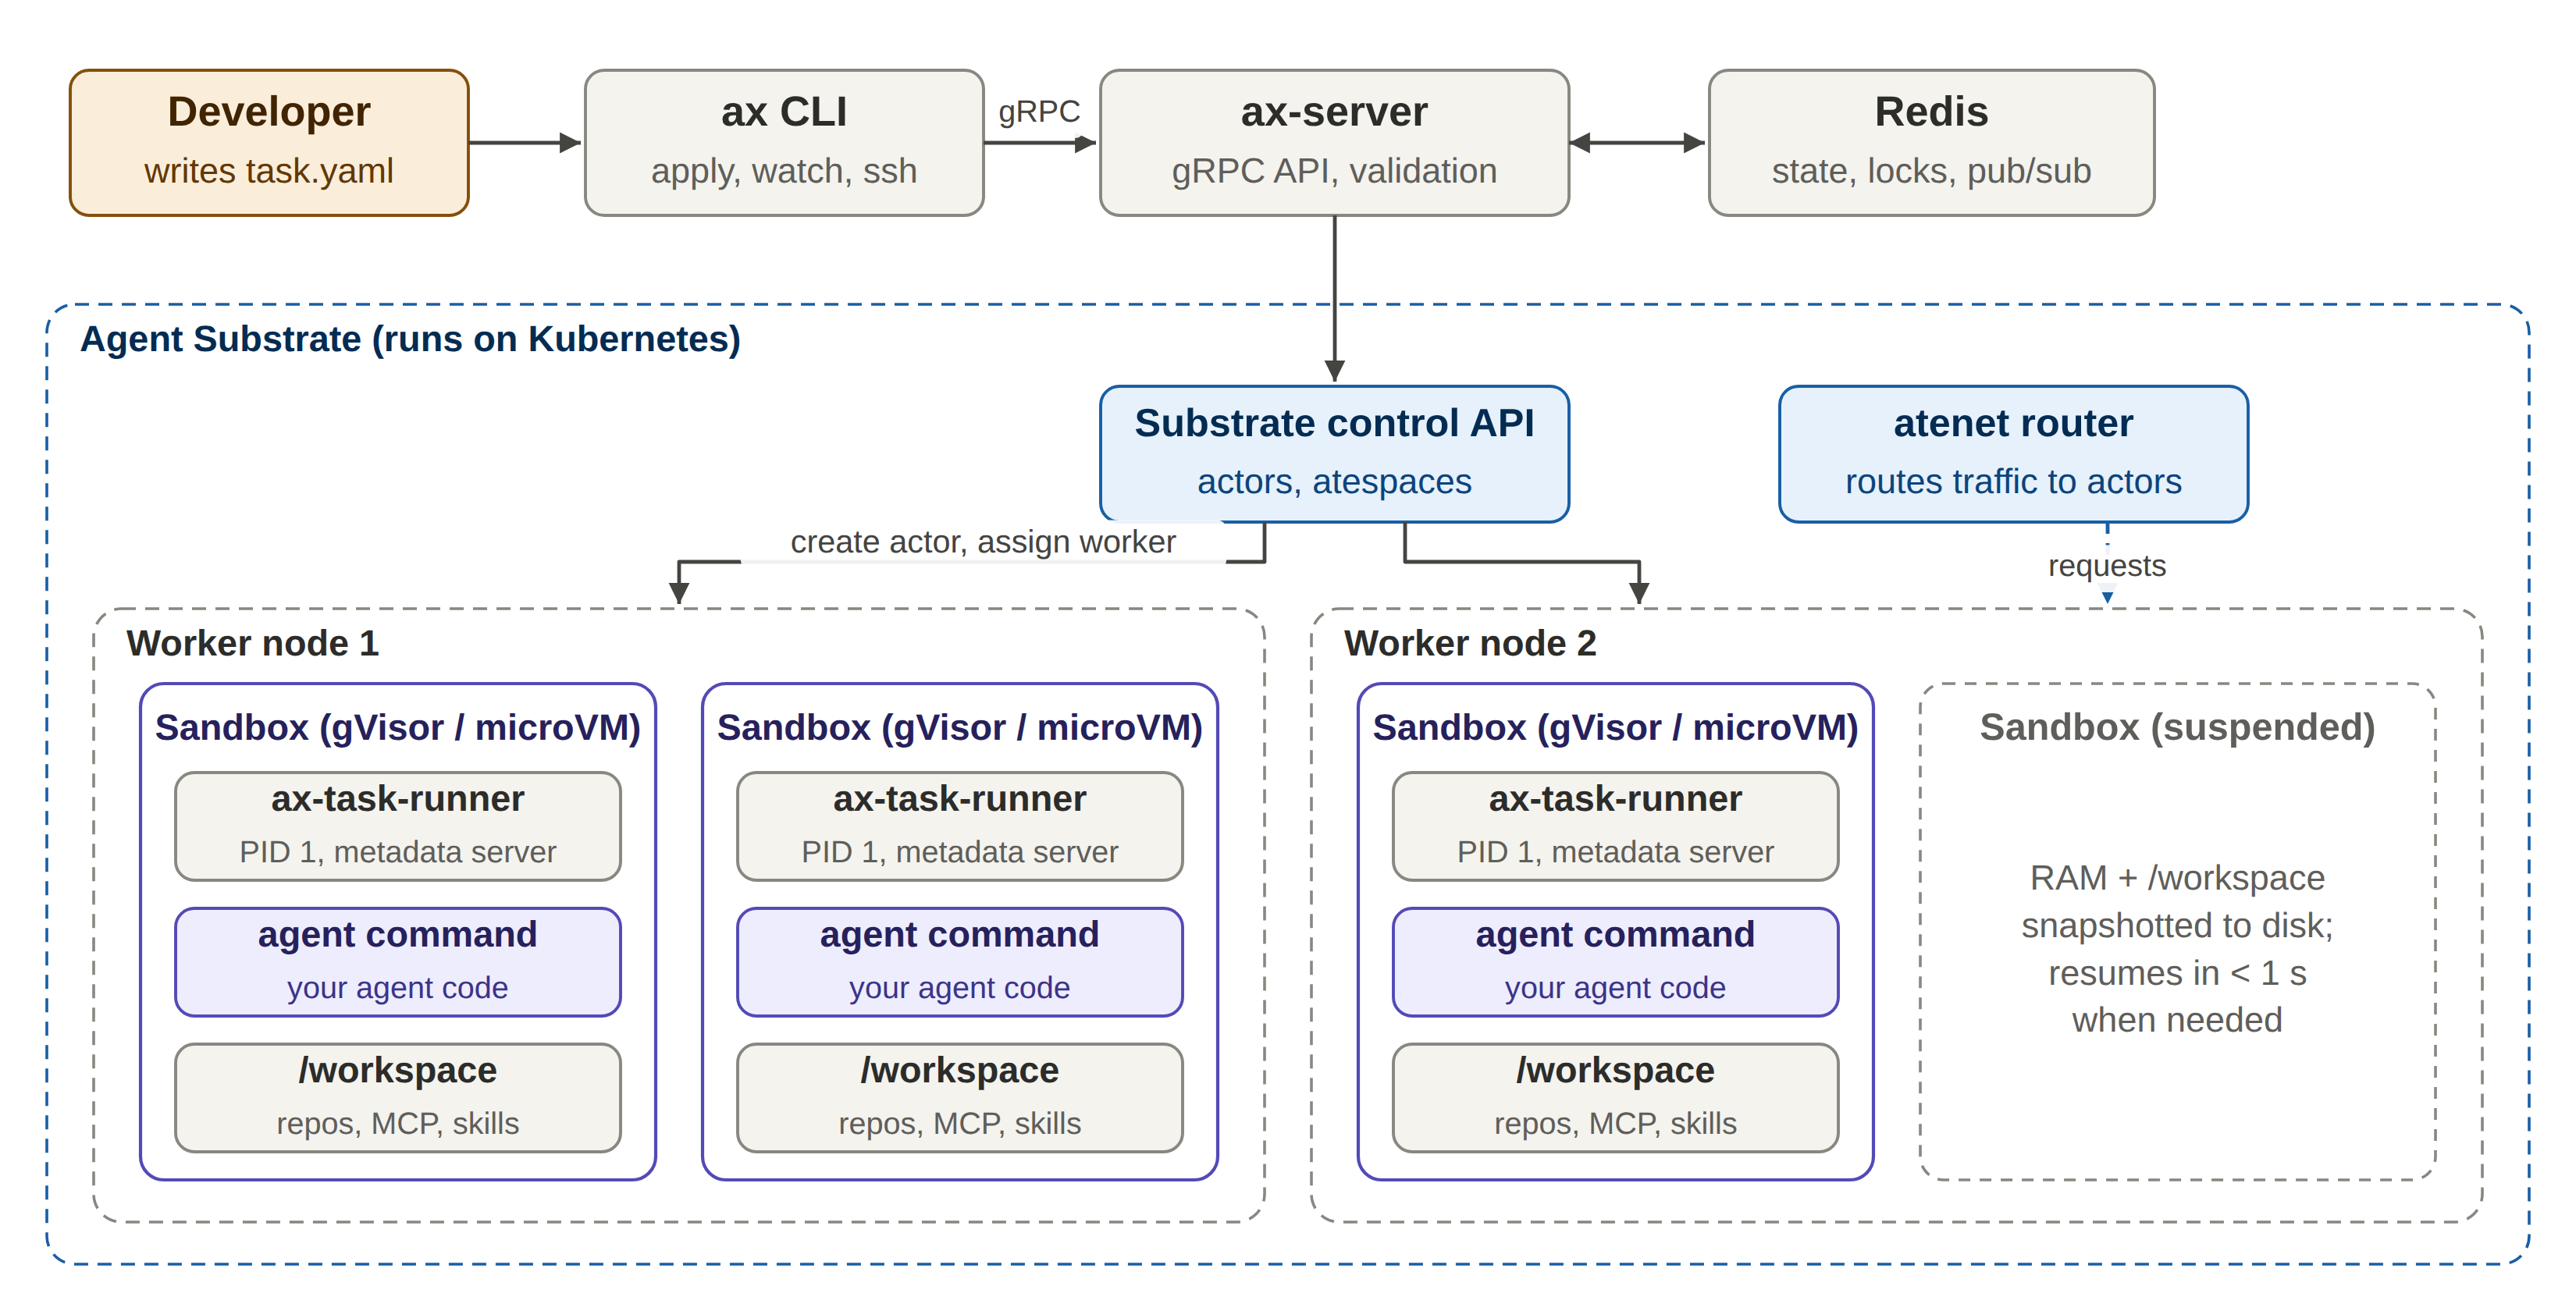
\includegraphics[width=\linewidth]{ax_architecture.png}
  \caption{AX architecture. The developer applies manifests with the \code{ax} CLI; \code{ax-server} persists them in Redis and asks Agent Substrate to create sandboxed actors on worker nodes. Each sandbox runs \code{ax-task-runner} as PID~1, the agent command, and a durable \code{/workspace} that survives suspension.}
  \label{fig:ax-arch}
\end{figure}

\subsubsection{Extension points that matter for us}

Three documented features let us add a KYA layer without changing AX:

\begin{enumerate}
  \item \textbf{The \code{--server} flag.} The CLI can be pointed at any gRPC endpoint that speaks the \code{ax.v1alpha1.AX} service. We can place our admission proxy there and forward accepted calls to the real \code{ax-server}.
  \item \textbf{Custom runners.} The runner contract is public: any image with an executable at \codeurl{/usr/local/bin/ax-task-runner} that serves \code{/healthz} and \code{/readyz} on port~80 is accepted. AX also exposes the runner as a Go package (\codeurl{github.com/google/ax/runner}) that can be embedded with extra logic~\cite{ax-runner}. Our KYA runner uses this.
  \item \textbf{The \code{SuspendTask} RPC.} Any authorised client can checkpoint and pause a task. Our trust observer uses it as an emergency brake.
\end{enumerate}

\begin{warnbox}[What AX does \emph{not} provide today]
The AX roadmap lists ``SPIFFE identity for tasks'', ``governance'' (access control, policy enforcement, budget guardrails, audit) and ``telemetry and trajectory collection'' as future work~\cite{ax-roadmap}. None of these exist in the current release. They are precisely the areas this project covers, which makes our work complementary to the project's own direction rather than competing with it.
\end{warnbox}

\subsection{Know Your Agent (KYA)}

KYC rules require banks to identify customers before serving them. KYA transfers this idea to software agents. There is no single KYA standard yet; identity-verification companies, payment networks and standards bodies each publish their own version~\cite{sumsub-kya,entrust-kya,vouched-kya,astrasync-kya}. Across these sources, four pillars recur (Figure~\ref{fig:pillars}).

\begin{figure}[H]
  \centering
  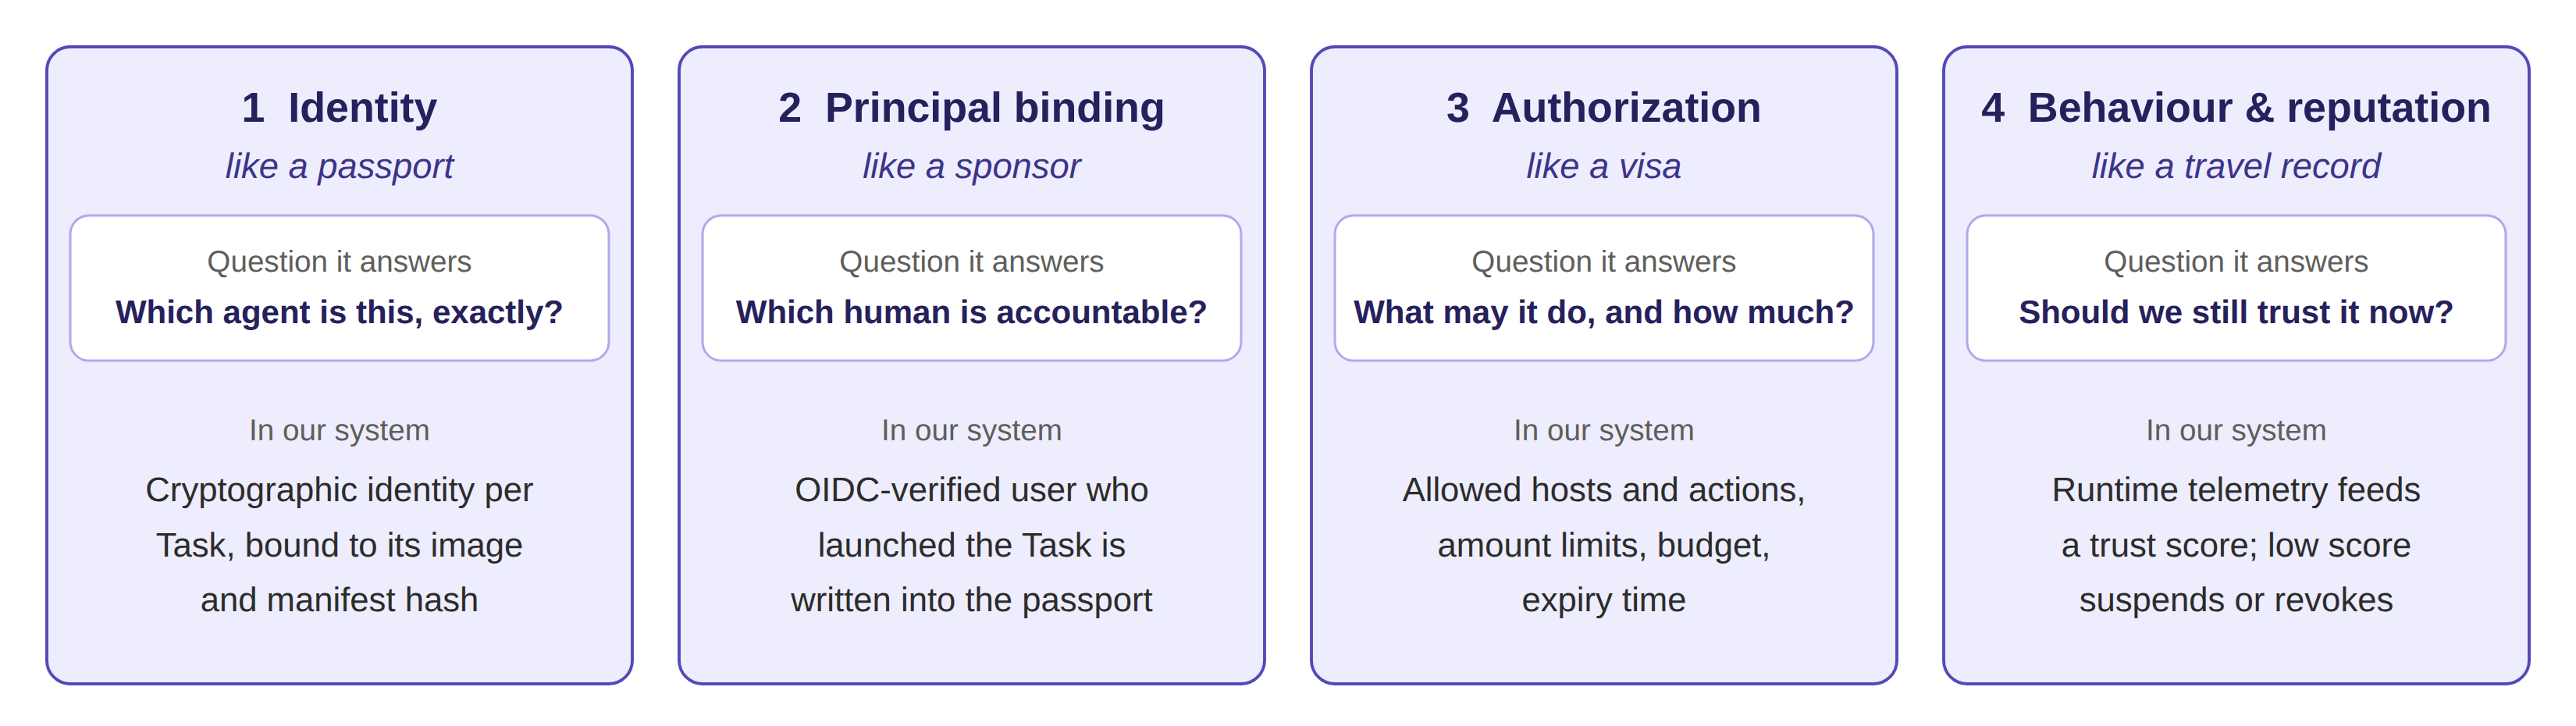
\includegraphics[width=\linewidth]{kya_pillars.png}
  \caption{The four pillars of Know Your Agent, the everyday analogy for each, and how AgentPassport implements it.}
  \label{fig:pillars}
\end{figure}

\begin{enumerate}
  \item \textbf{Identity.} The agent has a cryptographic identity that cannot be copied or forged, like a passport number backed by a chip.
  \item \textbf{Principal binding.} The identity is linked to a verified human or organisation who is accountable for it, like a sponsor on a visa application. Sumsub describes the goal as a clear chain of responsibility that leads from the agent to a verified human~\cite{sumsub-kya}.
  \item \textbf{Authorization.} The agent's permissions are explicit and limited: which services, which actions, how much money, until when. This is the visa.
  \item \textbf{Behaviour and reputation.} Trust is not granted once and forever. Runtime behaviour is monitored, and trust can be reduced or withdrawn, like a travel record that border control consults every time.
\end{enumerate}

\begin{example}[KYA in one sentence per pillar]
``This request comes from task \code{shop-7f3a} running image \code{sha256:3a0d\ldots} (\emph{identity}), launched by Alper, who logged in through university SSO (\emph{principal}), allowed to create orders of up to 500~TRY at \code{shop.example.com} until 11:12 (\emph{authorization}), and its behaviour over the last 14 minutes has been normal (\emph{reputation}).''
\end{example}

\subsection{Related standards and building blocks}\label{sec:standards}

We deliberately build on existing, well-specified mechanisms instead of inventing new cryptography. Table~\ref{tab:standards} lists them and where each is used.

\begin{table}[H]
\small
\begin{tabularx}{\linewidth}{@{}L{4.2cm}YL{3.4cm}@{}}
\toprule
\textbf{Standard / technique} & \textbf{What it is} & \textbf{Used in}\\
\midrule
JWT / JWS (RFC 7519, 7515) & Signed JSON tokens with standard claims (\code{iss}, \code{sub}, \code{exp}, \ldots). & Passport format\\
Proof of possession, \code{cnf} (RFC 7800) and JWK thumbprint (RFC 7638) & Binds a token to a key, so a stolen token is useless without the key. & Passport $\leftrightarrow$ gateway key\\
HTTP Message Signatures (RFC 9421)~\cite{rfc9421} & Signs selected parts of an HTTP request (method, authority, path, headers). & Egress gateway, verifier\\
Digest fields (RFC 9530) & \code{Content-Digest} header carrying a hash of the body. & Body integrity\\
Web Bot Auth (IETF drafts)~\cite{webbotauth} & Profile of RFC 9421 for identifying automated clients, with a \code{Signature-Agent} header pointing to a key directory. & Signature profile\\
SPIFFE / SVID~\cite{spiffe} & Standard format for workload identities (\code{spiffe://trust-domain/path}). & Agent identifier\\
OpenID Connect, device grant (RFC 8628) & Human login, including from a terminal. & Principal binding\\
OAuth 2.0 Token Exchange (RFC 8693) & Exchanging one token for a narrower one. & Delegation to sub-tasks\\
Biscuit tokens~\cite{biscuit} & Tokens that holders can only attenuate (restrict), never widen. & Delegation (alternative)\\
Agent Payments Protocol (AP2)~\cite{ap2} & Google's protocol for agent payments using signed ``mandates'' from users. & Inspiration for step-up approvals\\
OpenTelemetry & Vendor-neutral traces, metrics and logs. & Trust observer inputs\\
Isolation forest~\cite{iforest} & Unsupervised anomaly detection on feature vectors. & Trust observer scoring\\
\bottomrule
\end{tabularx}
\caption{Standards and techniques AgentPassport builds on.}
\label{tab:standards}
\end{table}
